\documentclass[../report.tex]{subfiles}
\graphicspath{{\subfix{../image/}}}

\begin{document}

\subsection{Pathfinding}

One of the requirements of the this project is the autonomy of the vehicle - the forklift.
Based on the sensor readings the forklift needs to do decisions. This is done in most of
the essential algorithms of the forklift. All these algorithms conclude in the pathfinding.

\subsubsection{The warehouse layout}

The pathfinding algorithm is tied to the layout of the warehouse.
In warehouse typically is split into several hallways with shelves
at the sides. Hence, the grid (the lines for the forklift) should mirror this
real life condition. The grid is hence constructed 
by one ``transportation layer'' - connecting the different hallways, and the 
hallways - leading from the transportation layer to the pallet spaces. 
For this prototype of the forklift it was decided 
to first demo the drop off of a pallet in one hallway. This grid an easily be 
drawn on even a table, which makes it easy to demo at, for example, TekExpo or 
the final presentation. Four pallet spaces were deemed enough for the demo, as the logic
does not change from this amount onwards.
Moreover, it is only slightly less complicated
than including several hallways as the decisions to find the palletspace are 
practically the same. Just hallway has to be logically determined. Thus, this one-hallway algorithm
can then be easily extended to include more then one hallway. Using the limitations of
the grid the decision making can be broken down to simple if-else conditions 
based on the current coordinates and the targeted coordinates. The simplifications
arise from the following advantages of the grid:

\begin{itemize}
    \item Pallet spaces are only at certain columns
    \item There is only one path to each pallet space
    \item One transportation layer/hallway
\end{itemize}

Here an image of the testing space. The warehouse in the back and a simple
line following track for testing tuning and the detection of intersections 
in the front:

\quad
\begin{center}
    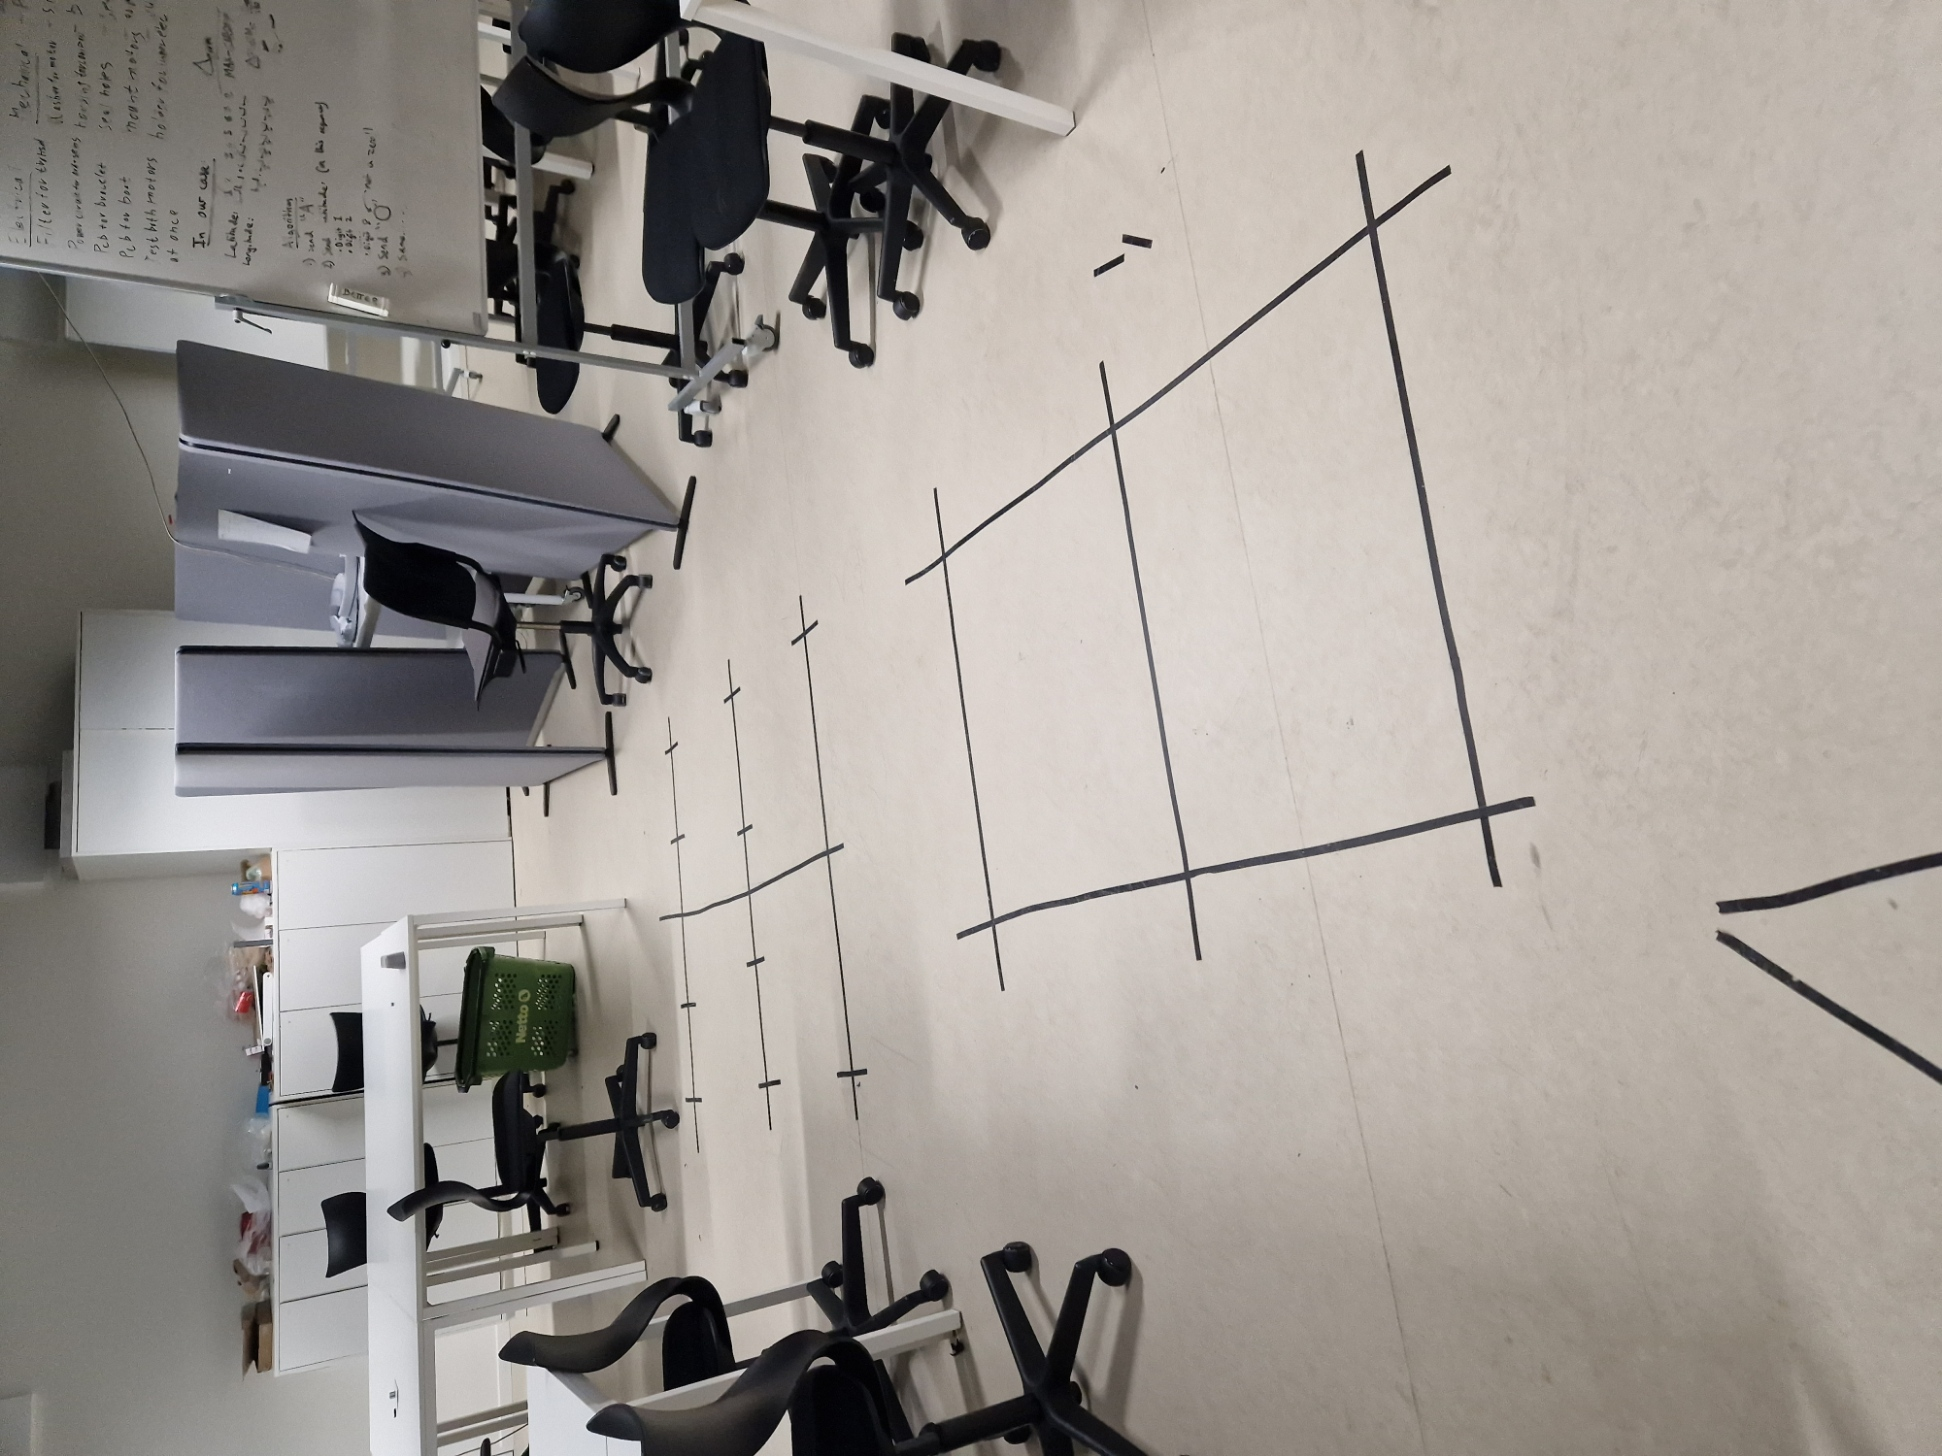
\includegraphics[width=0.6\textwidth, angle=-90]{testing_space.jpg}
\end{center}
\subsubsection{The actual algorithms}

In the following there are the two flowcharts. The single hallway algorithm
and the one for multiple hallways. It may be noted that this is only a 
high-level human representation, as the internal decision making is based
on the components described earlier - line-following, intersection detection, fork-control
etc..

\subsubsection{The warehouse algorithm for single hallway (symbolic / simplified)}
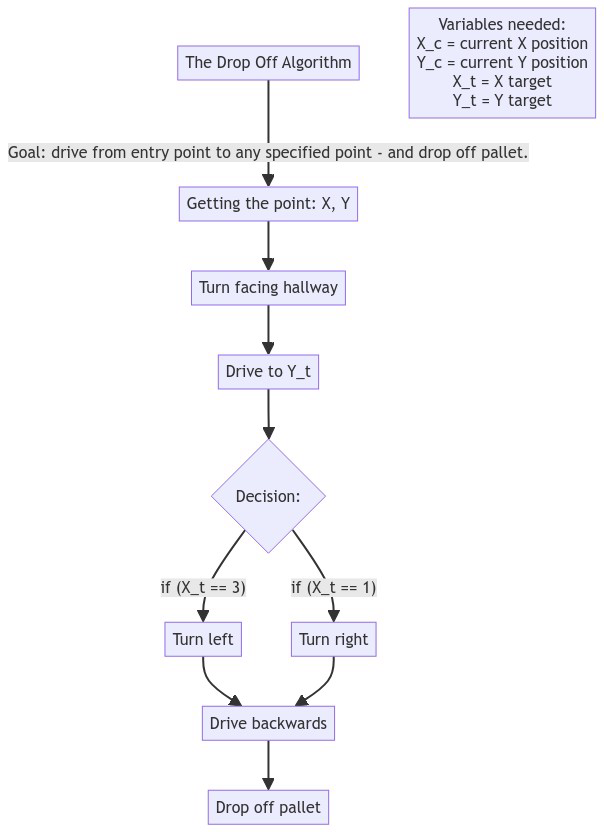
\includegraphics[width=\textwidth]{ThePalletDrop.md.1.png}
\subsubsection{The warehouse algorithm for multiple hallways}
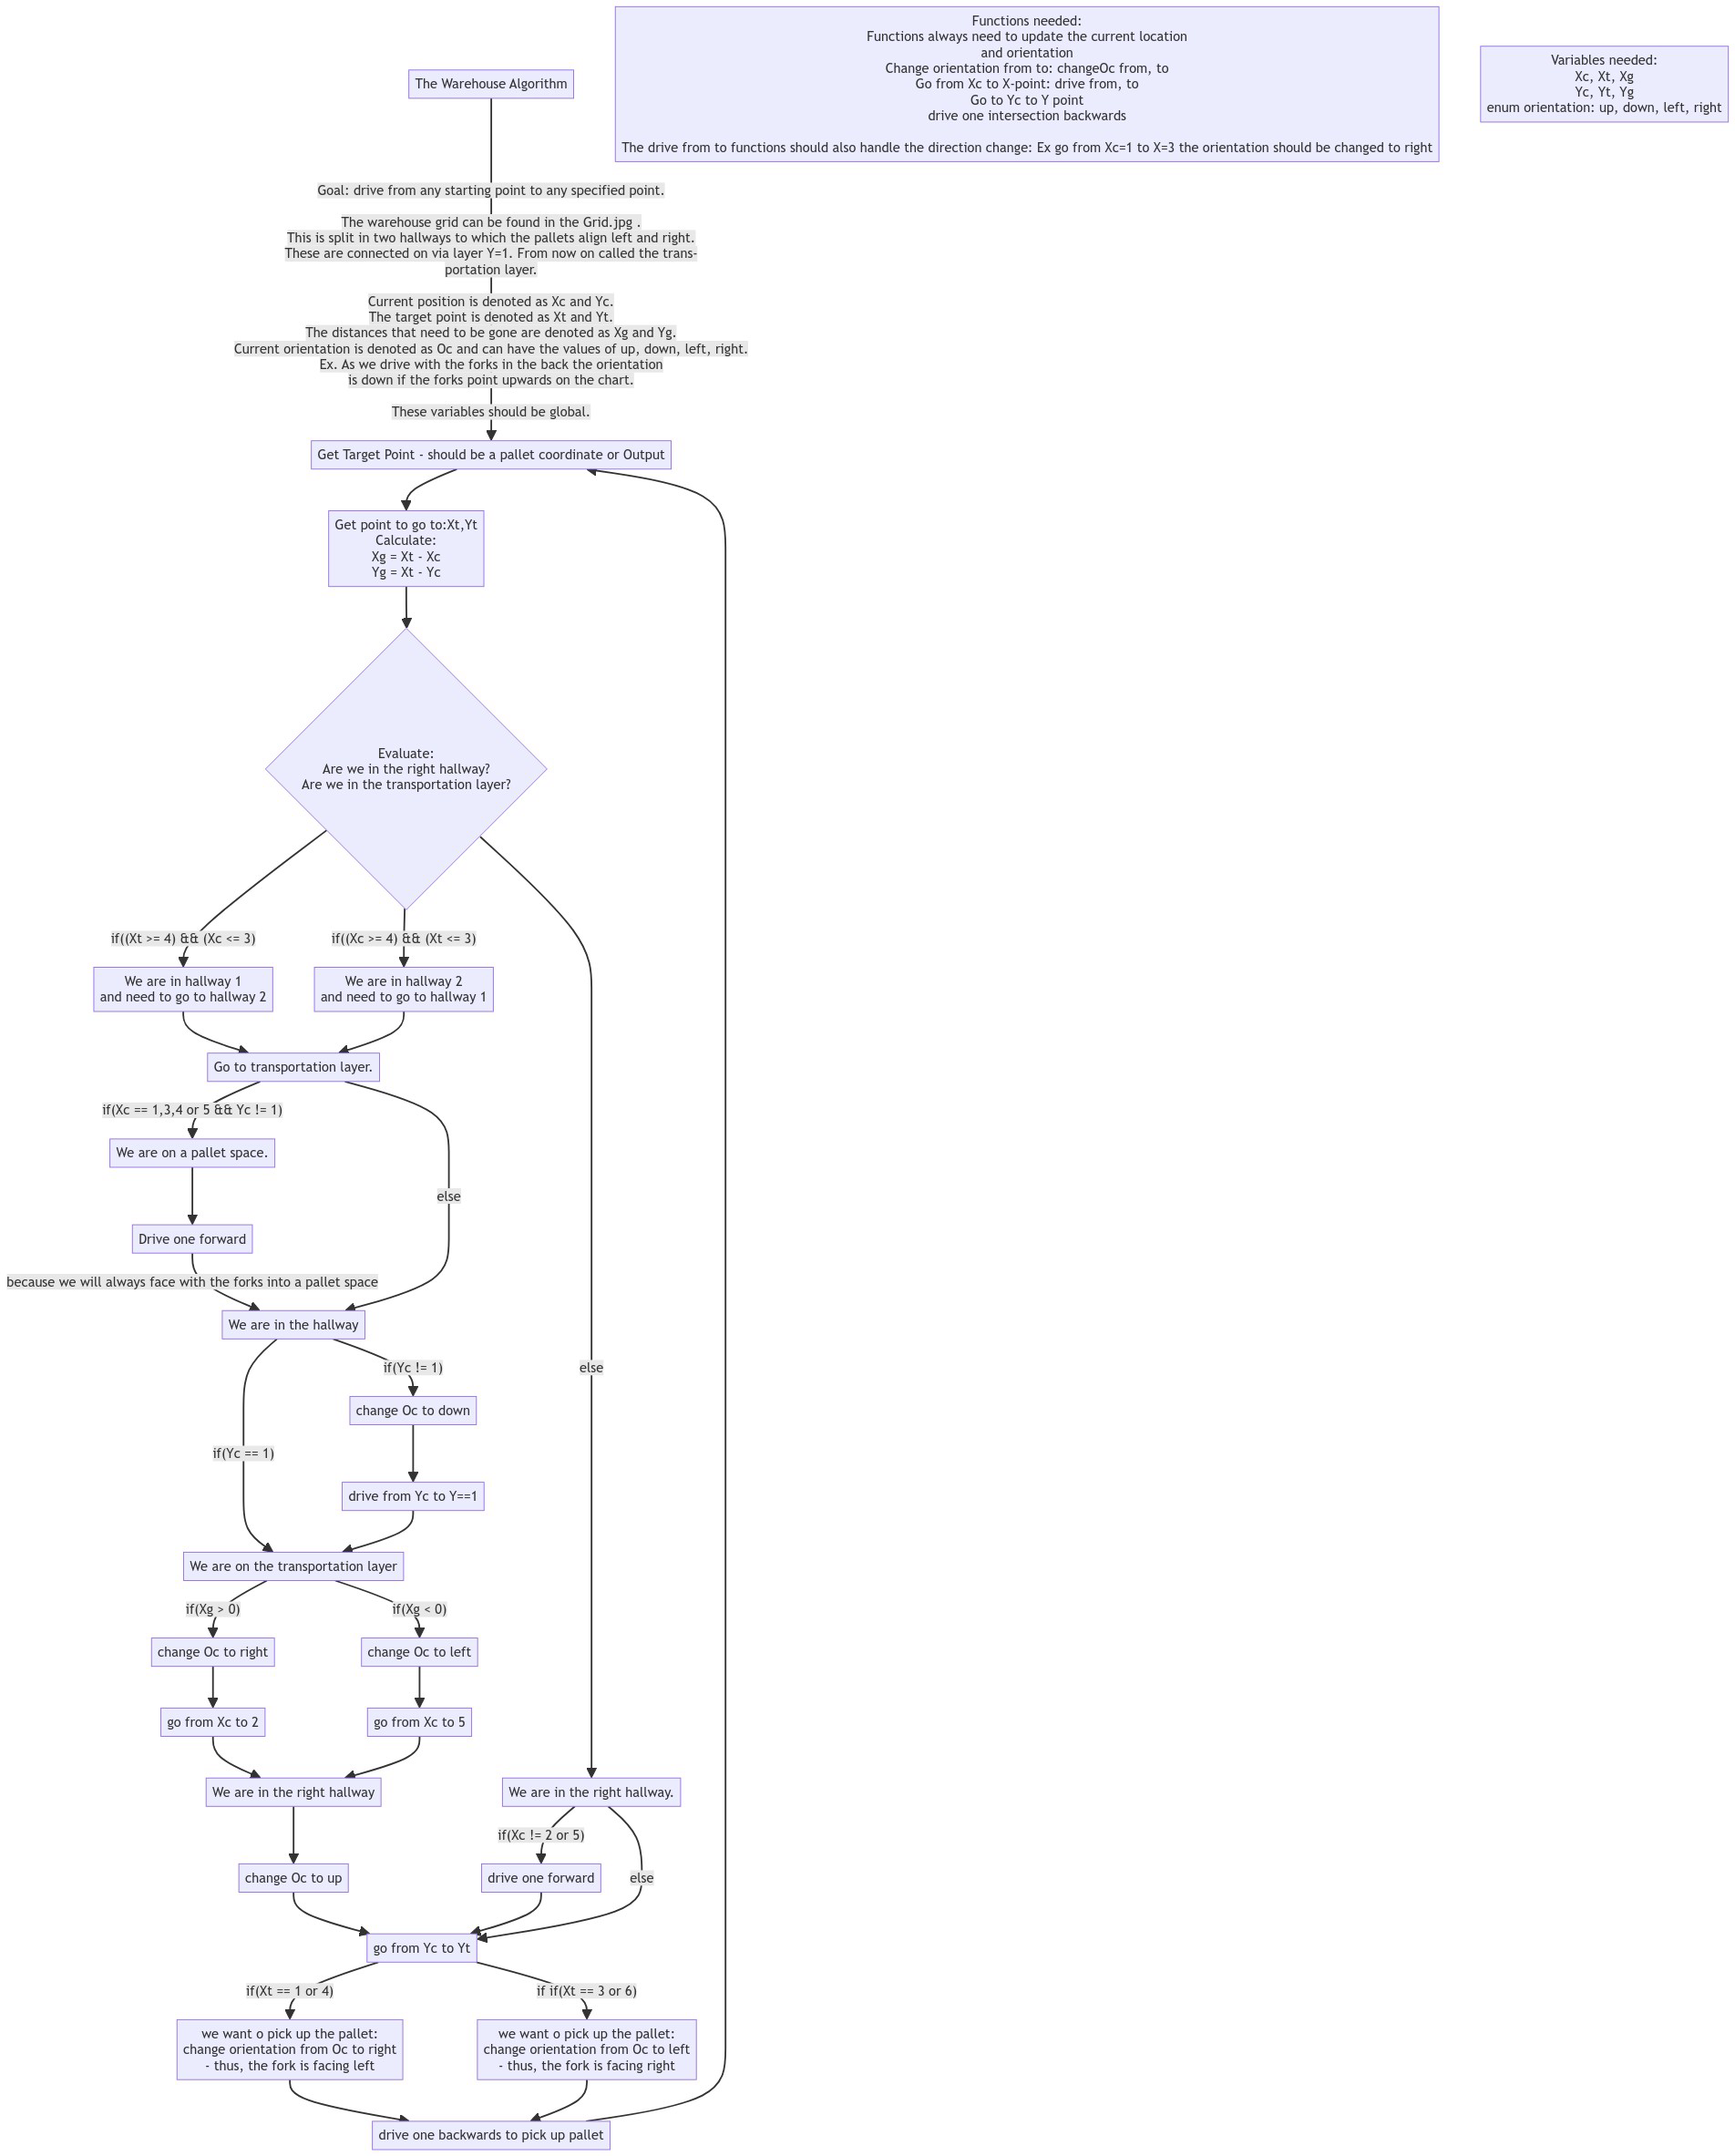
\includegraphics[width=\textwidth]{WarehouseAlgorithm.md.1.png}

\end{document}
